% !TeX program = xelatex
\documentclass[a4paper,10pt]{article}

% ============================================================================
% សន្លឹកកិច្ចការសិស្ស ស-ខ្មៅ (Student Fill-In Worksheet — No-LCD Classroom)
% មេរៀនទី១៦ (១៦.១)៖ លក្ខណៈមេដ្យាននៃត្រីកោណ (ត្រូវគ្នា ១០០% នឹង LS_Plan_MED.tex)
% ============================================================================
\usepackage[a4paper, left=0.95cm, right=0.95cm, top=0.75cm, bottom=0.90cm, footskip=0.48cm]{geometry}
\usepackage{amsmath}
\usepackage{unicode-math}
\usepackage{fontspec}
\usepackage{array, colortbl}
\usepackage[table]{xcolor}
\usepackage{enumitem}
\usepackage{pifont}
\usepackage{fancyhdr}
\usepackage{lastpage}
\usepackage{tikz}
\usepackage[most]{tcolorbox}
\usetikzlibrary{calc, arrows.meta, angles, quotes, decorations.markings, babel}

\makeatletter
\let\@expl@@@mark@update@singlecol@structures@@\relax
\makeatother

% ============================================================================
% ការកំណត់ពុម្ពអក្សរ (Cross-Platform Font Resolver)
% ============================================================================
\providecommand{\NGSFindFonts}{%
  \IfFileExists{C:/Windows/Fonts/cambria.ttc}{%
    \def\NGSSysPath{C:/Windows/Fonts/}%
    \def\NGSUserPath{C:/Users/KIT/AppData/Local/Microsoft/Windows/Fonts/}%
  }{%
    \IfFileExists{./fonts/KhmerOSsiemreap.ttf}{\def\NGSSysPath{./fonts/}\def\NGSUserPath{./fonts/}}{%
    \IfFileExists{../fonts/KhmerOSsiemreap.ttf}{\def\NGSSysPath{../fonts/}\def\NGSUserPath{../fonts/}}{%
    \IfFileExists{../../fonts/KhmerOSsiemreap.ttf}{\def\NGSSysPath{../../fonts/}\def\NGSUserPath{../../fonts/}}{%
    \IfFileExists{../../../fonts/KhmerOSsiemreap.ttf}{\def\NGSSysPath{../../../fonts/}\def\NGSUserPath{../../../fonts/}}{%
    \IfFileExists{../../../../fonts/KhmerOSsiemreap.ttf}{\def\NGSSysPath{../../../../fonts/}\def\NGSUserPath{../../../../fonts/}}{%
    \IfFileExists{../../../../../fonts/KhmerOSsiemreap.ttf}{\def\NGSSysPath{../../../../../fonts/}\def\NGSUserPath{../../../../../fonts/}}{%
    \IfFileExists{../../../../../../fonts/KhmerOSsiemreap.ttf}{\def\NGSSysPath{../../../../../../fonts/}\def\NGSUserPath{../../../../../../fonts/}}{%
      \def\NGSSysPath{../../../../../../../fonts/}\def\NGSUserPath{../../../../../../../fonts/}%
    }}}}}}}%
  }%
}
\NGSFindFonts

\setmathfont[Path={\NGSSysPath}, FontIndex=1, Scale=1.02]{cambria.ttc}
\defaultfontfeatures{Ligatures=TeX}

\setmainfont[
  Path={\NGSUserPath},
  Extension=.ttf,
  Script=Khmer,
  BoldFont={KhmerOSsiemreap},
  BoldFeatures={FakeBold=1.8},
  ItalicFont={KhmerOSsiemreap},
  ItalicFeatures={FakeSlant=0.25},
  BoldItalicFont={KhmerOSsiemreap},
  BoldItalicFeatures={FakeBold=1.8, FakeSlant=0.25}
]{KhmerOSsiemreap}

\newfontfamily\muol[Path={\NGSUserPath}, Extension=.ttf, Script=Khmer]{KhmerOSmuollight}
\newfontfamily\TimesEn[Path={\NGSSysPath}, Extension=.ttf, BoldFont={timesbd}, ItalicFont={timesi}, BoldItalicFont={timesbi}]{times}

\XeTeXlinebreaklocale "km"
\XeTeXlinebreakskip = 0pt plus 1pt minus 0.1pt

% ============================================================================
% ក្ដារពណ៌ ស-ខ្មៅ សម្រាប់បោះពុម្ពច្បាស់ ១០០%
% ============================================================================
\definecolor{panelgray}{gray}{0.93}
\definecolor{headgray}{gray}{0.85}

\pagestyle{fancy}
\fancyhf{}
\renewcommand{\headrulewidth}{0pt}
\fancyfoot[L]{\fontsize{8pt}{10pt}\selectfont អនុវិទ្យាល័យព្រះក្រសាំង \en{---} គណិតវិទ្យា ថ្នាក់ទី៨ \en{|} មេរៀនទី១៦ (១៦.១ លក្ខណៈមេដ្យាននៃត្រីកោណ)}
\fancyfoot[R]{\fontsize{8.2pt}{10pt}\selectfont ទំព័រ \en{\thepage\ / \pageref{LastPage}}}

\setlength{\parindent}{0pt}
\setlength{\parskip}{0pt}
\setlength{\tabcolsep}{4pt}

\newcommand{\en}[1]{{\TimesEn #1}}
\newcommand{\enbf}[1]{{\TimesEn\textbf{#1}}}
\newcommand{\unit}[1]{\,\text{\en{#1}}}
\newcommand{\cnum}[1]{\mbox{\fontsize{10pt}{12pt}\selectfont\ding{\numexpr181+#1\relax}}}
\newcommand{\chkbox}{\tikz[baseline=-0.15ex]\draw[black, line width=0.85pt] (0,0) rectangle (0.25cm,0.25cm);}
\newcommand{\blank}[1]{\makebox[#1]{\dotfill}}
\newcommand{\tri}[1]{\ensuremath{\triangle #1}}
\newcommand{\ang}[1]{\ensuremath{\angle #1}}

\newcommand{\secbar}[2]{%
  \vspace{3pt}%
  \begin{tcolorbox}[
    enhanced, sharp corners, colback=headgray, colframe=black,
    boxrule=0.9pt, boxsep=1pt, top=2.5pt, bottom=2.5pt, left=6pt, right=6pt,
    after skip=3pt
  ]
    {\muol\fontsize{9.2pt}{13.5pt}\selectfont #1}\hfill{\fontsize{8.3pt}{11.5pt}\selectfont\textbf{#2}}
  \end{tcolorbox}%
}

\tikzset{
  tk1/.style={postaction={decorate},decoration={markings,mark=at position 0.50 with {\draw[black, line width=0.95pt](0,-0.10)--(0,0.10);}}},
  tk2/.style={postaction={decorate},decoration={markings,
    mark=at position 0.45 with {\draw[black, line width=0.95pt](0,-0.10)--(0,0.10);},
    mark=at position 0.55 with {\draw[black, line width=0.95pt](0,-0.10)--(0,0.10);}}},
  tk3/.style={postaction={decorate},decoration={markings,
    mark=at position 0.42 with {\draw[black, line width=0.95pt](0,-0.10)--(0,0.10);},
    mark=at position 0.50 with {\draw[black, line width=0.95pt](0,-0.10)--(0,0.10);},
    mark=at position 0.58 with {\draw[black, line width=0.95pt](0,-0.10)--(0,0.10);}}}
}

\newcolumntype{L}[1]{>{\raggedright\arraybackslash}p{#1}}
\newcolumntype{C}[1]{>{\centering\arraybackslash}p{#1}}

\begin{document}
\fontsize{9.4pt}{13.8pt}\selectfont

% ============================================================================
% ទំព័រទី ១៖ ក្បាលសន្លឹកកិច្ចការ + E1 + E2 (វាស់ 1:1 & សម្រាយបញ្ជាក់) + E3 សង្ខេប
% ============================================================================
\begin{tcolorbox}[
  enhanced, sharp corners, colback=white, colframe=black,
  boxrule=1.1pt, boxsep=2pt, top=3pt, bottom=3pt, left=6pt, right=6pt, after skip=3pt
]
  \begin{center}
    {\muol\fontsize{10.5pt}{15pt}\selectfont សន្លឹកកិច្ចការសិស្ស \enbf{---} គណិតវិទ្យា ថ្នាក់ទី៨ \enbf{(}មេរៀនទី១៦ ៖ ១៦\enbf{.}១ លក្ខណៈមេដ្យាននៃត្រីកោណ\enbf{)}}\\[2pt]
    {\fontsize{8.8pt}{12pt}\selectfont
    ឈ្មោះសិស្ស / ដៃគូ៖ \blank{6.2cm} \hspace{0.2cm}
    ថ្នាក់៖ \blank{1.4cm} \hspace{0.2cm}
    ក្រុម៖ \blank{1.2cm} \hspace{0.2cm}
    កាលបរិច្ឆេទ៖ \blank{2.8cm}}
  \end{center}
\end{tcolorbox}

% --- E1 Engage ---
\begin{tcolorbox}[
  enhanced, sharp corners, colback=panelgray, colframe=black,
  boxrule=0.8pt, boxsep=1.5pt, top=2.5pt, bottom=2.5pt, left=6pt, right=6pt, after skip=3pt
]
  \textbf{បេសកកម្មទី១ (\en{E1 - Engage})៖ បន្ទះតុឈើរាងត្រីកោណជើងតែមួយ} \hfill {\footnotesize\textit{(ពេលបោះពុម្ព សូមជ្រើស \en{Actual Size 100\%})}}\\
  ជាងឈើចង់ដាក់ជើងទម្រតែមួយគត់ត្រង់ចំណុច $G$ ក្រោមបន្ទះតុរាងត្រីកោណ $\tri{ABC}$ ដើម្បីឱ្យបន្ទះតុមានលំនឹងមិនផ្អៀង ។\\
  $\blacktriangleright$ \textbf{ទស្សន៍ទាយមុនវាស់ (\en{Predict})៖} តើចំណុច $G$ ស្ថិតនៅចម្ងាយប៉ុន្មាននៃមេដ្យាន $AA'$ រាប់ពីកំពូល $A$? \hspace{0.3cm}
  \chkbox\ ពាក់កណ្ដាល ($\frac{1}{2}AA'$) \hspace{0.4cm}
  \chkbox\ ពីរភាគបី ($\frac{2}{3}AA'$) \hspace{0.4cm}
  \chkbox\ បីភាគបួន ($\frac{3}{4}AA'$)
\end{tcolorbox}

% --- E2 Explore Part A: 1:1 Measurement ---
\secbar{ផ្នែកទី១ \enbf{(}ក\enbf{)} ៖ ពិសោធន៍វាស់ស្ទង់ខ្នាតពិត \enbf{1:1} ដោយបន្ទាត់ក្រិត \enbf{(E2 - Explore)}}{ការងារជាដៃគូ \en{4 min}}

\noindent
\begin{minipage}[c]{7.7cm}
  \centering
  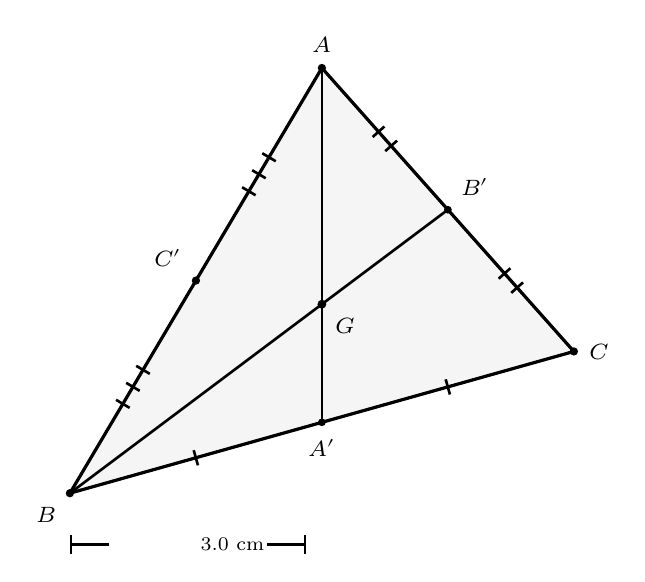
\begin{tikzpicture}[x=1cm, y=1cm, every node/.style={font=\footnotesize, text=black}]
    % ខ្នាតពិត 1:1 ៖ G=(0,0), A=(0,3.0), A'=(0,-1.5) => AA'=4.5 cm
    % B=(-3.2,-2.4), C=(3.2,-0.6) => B'=(1.6,1.2), BB'=6.0 cm, C'=(-1.6,0.3)
    \coordinate (G) at (0,0);
    \coordinate (A) at (0,3.0);
    \coordinate (Ap) at (0,-1.5);
    \coordinate (B) at (-3.2,-2.4);
    \coordinate (C) at (3.2,-0.6);
    \coordinate (Bp) at (1.6,1.2);
    \coordinate (Cp) at (-1.6,0.3);

    \fill[gray!8] (A) -- (B) -- (C) -- cycle;
    \draw[black, line width=1.15pt] (A) -- (B) -- (C) -- cycle;
    \draw[black, line width=0.95pt] (A) -- (Ap);
    \draw[black, line width=0.95pt] (B) -- (Bp);

    % សញ្ញាចំណុចកណ្ដាលជ្រុងទាំង ៣
    \draw[black, line width=0.8pt, tk1] (B) -- (Ap);
    \draw[black, line width=0.8pt, tk1] (Ap) -- (C);
    \draw[black, line width=0.8pt, tk2] (A) -- (Bp);
    \draw[black, line width=0.8pt, tk2] (Bp) -- (C);
    \draw[black, line width=0.8pt, tk3] (A) -- (Cp);
    \draw[black, line width=0.8pt, tk3] (Cp) -- (B);

    \fill[black] (A) circle (1.5pt) node[above=2pt] {$A$};
    \fill[black] (B) circle (1.5pt) node[below left=1.5pt] {$B$};
    \fill[black] (C) circle (1.5pt) node[right=2pt] {$C$};
    \fill[black] (Ap) circle (1.4pt) node[below=2.5pt] {$A'$};
    \fill[black] (Bp) circle (1.4pt) node[above right=1.5pt] {$B'$};
    \fill[black] (Cp) circle (1.5pt) node[above left=1.5pt] {$C'$};
    \fill[black] (G) circle (1.6pt) node[below right=1.5pt] {$G$};

    % បន្ទះផ្ទៀងខ្នាតពិត 3 cm
    \draw[black, line width=0.9pt, |-|] (-3.2,-3.05) -- (-0.2,-3.05)
      node[midway, fill=white, inner sep=1pt, font=\scriptsize] {បន្ទះផ្ទៀងខ្នាត \en{3.0 cm}};
  \end{tikzpicture}
\end{minipage}%
\hfill
\begin{minipage}[c]{11.0cm}
  \textbf{សេចក្ដីណែនាំអនុវត្តផ្ទាល់លើរូបខាងឆ្វេង៖}\\[2pt]
  $1.$ ប្រើបន្ទាត់ក្រិតភ្ជាប់កំពូល $C$ ទៅចំណុចកណ្ដាល $C'$ នៃជ្រុង $AB$ ។ តើមេដ្យានទីបី $CC'$ កាត់តាមចំណុចប្រសព្វ $G$ ដែរឬទេ? \hspace{0.2cm} \chkbox\ កាត់តាម $G$ \hspace{0.25cm} \chkbox\ មិនកាត់តាម\\[3pt]
  $2.$ វាស់ប្រវែងពិតគិតជាសង់ទីម៉ែត្រ (\en{cm}) រួចបំពេញតារាងខាងក្រោម៖\\[3pt]
  {\renewcommand{\arraystretch}{1.46}
  \begin{tabular}{|C{1.45cm}|C{1.95cm}|C{1.95cm}|C{1.95cm}|C{2.05cm}|}
    \hline
    \cellcolor{headgray}\textbf{មេដ្យាន} & \cellcolor{headgray}\textbf{ប្រវែងសរុប} & \cellcolor{headgray}\textbf{ពីកំពូលទៅ $G$} & \cellcolor{headgray}\textbf{ពី $G$ ទៅជើង} & \cellcolor{headgray}\textbf{ផលធៀប} \\
    \hline
    $AA'$ & $AA'=\blank{0.85cm}$ & $AG=\blank{0.85cm}$ & $GA'=\blank{0.85cm}$ & $\frac{AG}{AA'}=\blank{0.85cm}$ \\
    \hline
    $BB'$ & $BB'=\blank{0.85cm}$ & $BG=\blank{0.85cm}$ & $GB'=\blank{0.85cm}$ & $\frac{BG}{BB'}=\blank{0.85cm}$ \\
    \hline
  \end{tabular}}\\[4pt]
  $3.$ \textbf{សង្កេត (\en{Observe})៖} ប្រៀបធៀប $AG$ និង $GA'$៖ គេឃើញ $AG = \blank{0.9cm} \times GA'$ ហើយ $GA' = \dfrac{\blank{0.6cm}}{\blank{0.6cm}}\,AA'$ និង $AG = \dfrac{\blank{0.6cm}}{\blank{0.6cm}}\,AA'$ ។
\end{minipage}

\vspace{3pt}
% --- E2 Explore Part B: Subgoal-Labeled Proof ---
\secbar{ផ្នែកទី១ \enbf{(}ខ\enbf{)} ៖ សម្រាយបញ្ជាក់ឧទាហរណ៍សៀវភៅគោល ទំព័រ ២០៥\,\enbf{--}\,២០៦ \enbf{(Subgoal Proof)}}{ការងារជាដៃគូ \en{7 min}}

\noindent
\begin{minipage}[c]{12.2cm}
  គេឱ្យ $\tri{ABC}$ មានមេដ្យាន $BB'$ និង $CC'$ កាត់គ្នាត្រង់ $G$ ។ តាង $D$ ជាចំណុចឆ្លុះនៃ $A$ ធៀបនឹង $G$ ។ ចូរបំពេញចន្លោះតាមជំហានរងទាំង ៤ ៖\\[3pt]
  $\bullet$ \textbf{ជំហានទី១ (ពិនិត្យ $\tri{ABD}$)៖} ដោយ $D$ ឆ្លុះនឹង $A$ ធៀបនឹង $G$ នោះ $G$ ជាចំណុចកណ្ដាលនៃអង្កត់ \blank{1.2cm} ($AG=GD$) ។ ក្នុង $\tri{ABD}$ មាន $C'$ ជាចំណុចកណ្ដាលនៃ $AB$ និង $G$ ជាចំណុចកណ្ដាលនៃ $AD$ នាំឱ្យបន្ទាត់ $C'G \parallel \blank{1.1cm}$ ឬ $CG \parallel BD \quad (1)$ ។\\[2.5pt]
  $\bullet$ \textbf{ជំហានទី២ (ពិនិត្យ $\tri{ACD}$)៖} ក្នុង $\tri{ACD}$ មាន $G$ ជាចំណុចកណ្ដាលនៃ $AD$ និង $B'$ ជាចំណុចកណ្ដាលនៃ \blank{1.1cm} នាំឱ្យ $GB' \parallel \blank{1.1cm}$ ឬ $GB \parallel CD \quad (2)$ ។\\[2.5pt]
  $\bullet$ \textbf{ជំហានទី៣ (ប្រសព្វមេដ្យាន)៖} តាម $(1)$ និង $(2)$ ចតុកោណ $BDCG$ ជា \blank{2.6cm} នាំឱ្យអង្កត់ទ្រូង $BC$ និង $GD$ កាត់គ្នាត្រង់ចំណុចកណ្ដាលរួម $A'$ ។ ដូចនេះមេដ្យាន $AA'$ កាត់តាមចំណុច \blank{0.9cm} ។\\[2.5pt]
  $\bullet$ \textbf{ជំហានទី៤ (ផលធៀបប្រវែង)៖} ដោយ $A'$ កណ្ដាល $GD \Rightarrow GD = 2\blank{1.0cm}$ តែ $AG=GD \Rightarrow AG = 2\blank{1.0cm}$ ។ ដោយ $AA'=AG+GA'=\blank{0.8cm}\,GA'$ គេទាញបាន $GA'=\dfrac{\blank{0.6cm}}{\blank{0.6cm}}\,AA'$ និង $AG=\dfrac{\blank{0.6cm}}{\blank{0.6cm}}\,AA'$ ។
\end{minipage}%
\hfill
\begin{minipage}[c]{6.5cm}
  \centering
  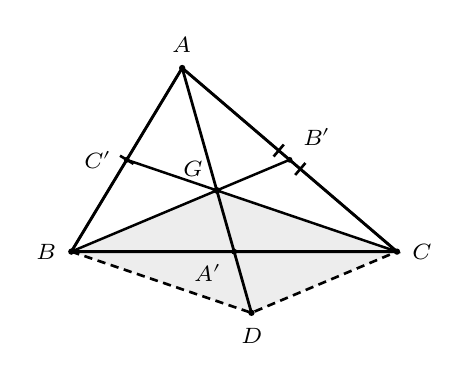
\begin{tikzpicture}[scale=0.88, every node/.style={font=\footnotesize, text=black}]
    \coordinate (A) at (-0.55,2.65);
    \coordinate (B) at (-2.15,0);
    \coordinate (C) at (2.55,0);
    \coordinate (Ap) at ($(B)!0.5!(C)$);
    \coordinate (Bp) at ($(A)!0.5!(C)$);
    \coordinate (Cp) at ($(A)!0.5!(B)$);
    \coordinate (G) at ($0.3333*(A)+0.3333*(B)+0.3333*(C)$);
    \coordinate (D) at ($2*(G)-(A)$);

    \fill[gray!14] (B) -- (D) -- (C) -- (G) -- cycle;
    \draw[black, line width=1.05pt] (A) -- (B) -- (C) -- cycle;
    \draw[black, line width=0.9pt] (B) -- (Bp) (C) -- (Cp);
    \draw[black, line width=1.0pt] (A) -- (D);
    \draw[black, line width=0.95pt, densely dashed] (B) -- (D) -- (C);
    \draw[black, line width=0.8pt, tk1] (A) -- (Cp) (Cp) -- (B);
    \draw[black, line width=0.8pt, tk2] (A) -- (Bp) (Bp) -- (C);

    \fill[black] (A) circle (1.3pt) node[above=2pt] {$A$};
    \fill[black] (B) circle (1.3pt) node[left=2pt] {$B$};
    \fill[black] (C) circle (1.3pt) node[right=2pt] {$C$};
    \fill[black] (Cp) circle (1.2pt) node[left=2pt] {$C'$};
    \fill[black] (Bp) circle (1.2pt) node[above right=1.5pt] {$B'$};
    \fill[black] (Ap) circle (1.2pt) node[below left=1pt] {$A'$};
    \fill[black] (G) circle (1.4pt) node[above left=1.5pt] {$G$};
    \fill[black] (D) circle (1.3pt) node[below=2pt] {$D$};
  \end{tikzpicture}
\end{minipage}

\vspace{3pt}
% --- E3 Explain: Theorem & Warrant Bank ---
\secbar{ផ្នែកទី២ ៖ បញ្ញត្តិទ្រឹស្តីបទ និងធនាគារហេតុផល \enbf{(E3 - Explain)}}{សង្ខេបរួមគ្នា \en{6 min}}

\begin{tcolorbox}[
  enhanced, sharp corners, colback=white, colframe=black,
  boxrule=0.9pt, boxsep=2.5pt, top=3.5pt, bottom=3.5pt, left=6pt, right=6pt
]
  $\bullet$ \textbf{ទ្រឹស្តីបទ (ទំ.២០៦)៖} មេដ្យានទាំងបីនៃត្រីកោណមួយប្រសព្វគ្នាត្រង់ចំណុចតែមួយដែលឋិតនៅចម្ងាយ \textbf{«\blank{2.2cm}»} នៃមេដ្យាននីមួយៗពីកំពូល ។ ចំណុចនេះហៅថា \textbf{\blank{3.2cm}} នៃត្រីកោណ ហើយកំណត់ដោយអក្សរ \blank{0.9cm} ។\\[3pt]
  $\bullet$ \textbf{រូបមន្តប្រើញឹកញាប់៖} $AG = \dfrac{2}{3}AA' \quad;\quad GA' = \dfrac{1}{3}AA' \quad;\quad AG = 2GA' \quad;\quad BG = \dfrac{2}{3}BB' \quad;\quad CG = \dfrac{2}{3}CC'$ ។\\[3pt]
  $\bullet$ \textbf{ចំណាំប្រុងប្រយ័ត្ន៖} ចម្ងាយពីកំពូលទៅ $G$ ស្មើនឹង \textbf{២ ដង} នៃចម្ងាយពី $G$ ទៅជើងមេដ្យានជានិច្ច (កុំច្រឡំ $\frac{2}{3}$ ជាមួយ $\frac{1}{2}$!) ។\\[3pt]
  $\bullet$ \textbf{ធនាគារហេតុផល (\en{Warrant Bank})៖}
  \cnum{1} និយមន័យមេដ្យាន ($A'B=A'C$) \;\textbar\;
  \cnum{2} បាតមធ្យមត្រីកោណ \;\textbar\;
  \cnum{3} អង្កត់ទ្រូងប្រលេឡូក្រាម \;\textbar\;
  \cnum{4} ទ្រឹស្ដីបទទីប្រជុំទម្ងន់ $G$ \;\textbar\;
  \cnum{5} លក្ខណៈមេដ្យាទ័រ ($MB=MC$)
\end{tcolorbox}

\newpage

% ============================================================================
% ទំព័រទី ២៖ E4 (លំហាត់គំរូបន្ថយជំហាន + ប្រតិបត្តិសង់ C) + E5 (វិភាគកំហុស & Exit) + កិច្ចការផ្ទះ
% ============================================================================

\secbar{ផ្នែកទី៣ ៖ ពង្រីកចំណេះដឹង \enbf{---} លំហាត់គំរូបន្ថយជំហាន និងប្រតិបត្តិសង់រូប \enbf{(E4 - Elaborate)}}{អនុវត្ត \en{10 min}}

\noindent
\begin{minipage}[t]{10.4cm}\vspace{0pt}
  \begin{tcolorbox}[
    enhanced, sharp corners, colback=white, colframe=black, equal height group=rowE4,
    boxrule=0.85pt, boxsep=2pt, top=3pt, bottom=3pt, left=5pt, right=5pt
  ]
    \textbf{៣.ក លំហាត់គំរូបន្ថយជំហាន (សៀវភៅគោល ទំ.២០៦)៖}\\
    ឧបមាថាក្នុង $\tri{ABC}$ មេដ្យានគូសចេញពីកំពូល $B$ និង $C$ មានប្រវែងស្មើគ្នា ($BB'=CC'$) ។ ចូរបំពេញចន្លោះ និងលេខហេតុផល \cnum{1}--\cnum{5} ៖\\[3pt]
    \textbf{ក. បង្ហាញថាទីប្រជុំទម្ងន់ $G$ ស្ថិតលើមេដ្យាទ័រនៃអង្កត់ $BC$៖}\\
    -- តាង $A', B', C'$ ជាជើងមេដ្យានគូសចេញពី $A, B, C$ នៃ $\tri{ABC}$ ។\\
    -- ដោយ $G$ ជាទីប្រជុំទម្ងន់នៃ $\tri{ABC}$ (ហេតុផល \blank{0.9cm}) គេបាន៖\\
    \hspace*{0.4cm}$GB = \dfrac{\blank{0.6cm}}{\blank{0.6cm}}\,BB'$ \quad និង \quad $GC = \dfrac{\blank{0.6cm}}{\blank{0.6cm}}\,CC'$ ។\\
    -- តែ $BB' = CC'$ (សម្មតិកម្ម) នាំឱ្យគេបាន $GB = \blank{1.2cm}$ ។\\
    -- តាមហេតុផល \blank{0.9cm} ចំណុច $G$ ស្ថិតនៅស្មើចម្ងាយពី $B$ និង $C$ ដូចនេះ $G$ ស្ថិតនៅលើ \blank{2.8cm} នៃអង្កត់ $BC$ ។\\[4pt]
    \textbf{ខ. ទាញបញ្ជាក់ថា $\tri{ABC}$ ជាត្រីកោណសមបាតកំពូល $A$៖}\\
    -- ដោយ $A'$ ជាជើងមេដ្យាន នោះ $A'B = \blank{1.1cm}$ (ហេតុផល \blank{0.9cm}) នាំឱ្យ $A'$ ក៏ស្ថិតលើមេដ្យាទ័រនៃ $BC$ ដែរ ។\\
    -- ដូចនេះបន្ទាត់មេដ្យាន $AA'$ (ឬ $AG$) ជា \blank{2.6cm} នៃអង្កត់ $BC$ ។\\
    -- ដោយកំពូល $A$ ស្ថិតលើមេដ្យាទ័រនៃ $BC$ នាំឱ្យ $AB = \blank{1.2cm}$ ។\\
    -- ដូចនេះ $\tri{ABC}$ ជាត្រីកោណ \blank{3.2cm} ។
  \end{tcolorbox}
\end{minipage}%
\hfill
\begin{minipage}[t]{8.4cm}\vspace{0pt}
  \begin{tcolorbox}[
    enhanced, sharp corners, colback=white, colframe=black, equal height group=rowE4,
    boxrule=0.85pt, boxsep=2pt, top=3pt, bottom=3pt, left=5pt, right=5pt
  ]
    \textbf{៣.ខ ប្រតិបត្តិ (ទំ.២០៦)៖ សង់កំពូល $C$ នៃ $\tri{ABC}$}\\
    គេស្គាល់កំពូល $A, B$ និងបន្ទាត់មេដ្យានពីរ $d$ (តាម $A$), $d'$ (តាម $B$) ។ ចូរសង់ចំណុច $C$ ដោយបន្ទាត់និងដែកឈានលើរូបខាងក្រោម៖\\[2pt]
    \begin{center}
      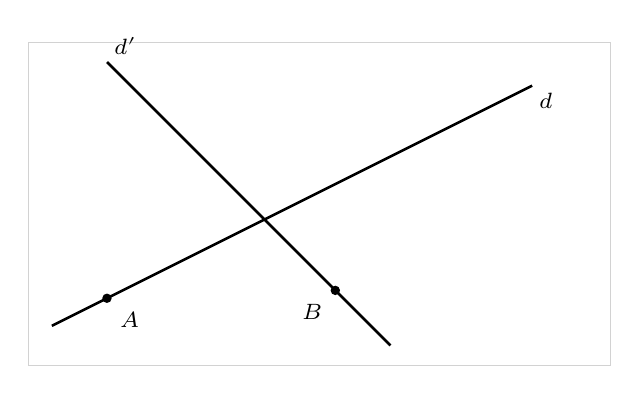
\begin{tikzpicture}[x=1cm, y=1cm, every node/.style={font=\footnotesize, text=black}]
        \draw[gray!35, line width=0.4pt] (-2.6,-0.5) rectangle (4.8,3.6);
        \coordinate (G2) at (0.4,1.35);
        \coordinate (A2) at (-1.6,0.35);
        \coordinate (B2) at (1.3,0.45);
        \draw[black, line width=0.95pt] (-2.3,0.0) -- (3.8,3.05) node[below right=-1pt] {$d$};
        \draw[black, line width=0.95pt] (2.0,-0.25) -- (-1.6,3.35) node[above right=-1pt] {$d'$};
        \fill[black] (A2) circle (1.7pt) node[below right=1.5pt] {$A$};
        \fill[black] (B2) circle (1.7pt) node[below left=1.5pt] {$B$};
      \end{tikzpicture}
    \end{center}
    \vspace{-2pt}
    \textbf{សង្ខេបជំហានសង់ទាំង ៣៖}\\
    $1.$ ដៅចំណុចប្រសព្វ $G = d \cap d'$ (ជា \blank{2.5cm}) ។\\
    $2.$ លើបន្ទាត់ $d$ ដៅជើងមេដ្យាន $A'$ ឱ្យ $GA' = \frac{1}{2}\blank{1.0cm}$ ។\\
    $3.$ គូសកន្លះបន្ទាត់ $BA'$ យក $A'C = \blank{1.1cm}$ បានកំពូល $C$ ។
  \end{tcolorbox}
\end{minipage}

% --- E5 Evaluate: Error Analysis + Calculation + Exit Check ---
\secbar{ផ្នែកទី៤ ៖ វាយតម្លៃលទ្ធផលសិក្សា \enbf{---} វិភាគកំហុស និងសំណួរត្រួតពិនិត្យរហ័ស \enbf{(E5 - Evaluate)}}{ធ្វើដោយឯករាជ្យ \en{10 min}}

\noindent
\begin{minipage}[t]{10.4cm}\vspace{0pt}
  \begin{tcolorbox}[
    enhanced, sharp corners, colback=white, colframe=black, equal height group=rowE5,
    boxrule=0.85pt, boxsep=2pt, top=3pt, bottom=3pt, left=5pt, right=5pt
  ]
    \textbf{៤.ក លំហាត់វិភាគកំហុស (\en{Error Diagnosis})៖}\\
    ក្នុង $\tri{MNP}$ មានទីប្រជុំទម្ងន់ $G$ និងមេដ្យានពីរគឺ $MI = 12\unit{cm}$ ព្រមទាំង $NJ$ ដែលមាន $GN = 5\unit{cm}$ ។\\
    សិស្សម្នាក់បានគណនាខុសដូចតទៅ៖\\
    \hspace*{0.3cm}{\itshape «គេបាន $MG = \frac{1}{2}MI = 6\unit{cm}$ និង $NJ = 2GN = 10\unit{cm}$ ។»}\\[3pt]
    $\blacktriangleright$ \textbf{ចូររកកំហុស ហើយគណនាឡើងវិញឱ្យបានត្រឹមត្រូវ៖}\\
    $1.$ មូលហេតុដែលខុស៖ \blank{6.8cm}\\[3pt]
    $2.$ កែតម្រូវចំពោះមេដ្យាន $MI = 12\unit{cm}$៖\\
    \hspace*{0.3cm}$MG = \dfrac{\blank{0.6cm}}{\blank{0.6cm}}\,MI = \blank{2.0cm}$ \quad;\quad $GI = \blank{2.0cm}$ ។\\[3pt]
    $3.$ កែតម្រូវចំពោះមេដ្យាន $NJ$ (ស្គាល់ $GN = 5\unit{cm}$)៖\\
    \hspace*{0.3cm}ដោយ $GN = \dfrac{2}{3}NJ \Rightarrow NJ = \dfrac{3}{2}GN = \blank{2.2cm}$ \;;\; $GJ = \blank{1.8cm}$ ។
  \end{tcolorbox}
\end{minipage}%
\hfill
\begin{minipage}[t]{8.4cm}\vspace{0pt}
  \begin{tcolorbox}[
    enhanced, sharp corners, colback=white, colframe=black, equal height group=rowE5,
    boxrule=0.85pt, boxsep=2pt, top=3pt, bottom=3pt, left=5pt, right=5pt
  ]
    \textbf{៤.ខ សំណួរត្រួតពិនិត្យរហ័ស (\en{Exit Check})៖}\\
    ចូរគូសវង់ជុំវិញអក្សរនៃចម្លើយត្រឹមត្រូវតែមួយគត់៖\\[3pt]
    \textbf{សំណួរទី១៖} បើ $G$ ជាទីប្រជុំទម្ងន់នៃ $\tri{ABC}$ ($AA'$ ជាមេដ្យាន) ហើយប្រវែងពី $G$ ទៅជើងមេដ្យានគឺ $GA' = 4\unit{cm}$ តើប្រវែង $AG$ និង $AA'$ ស្មើប៉ុន្មាន?\\
    \hspace*{0.2cm}\textbf{ក.} $AG=4\unit{cm},\; AA'=8\unit{cm}$\\
    \hspace*{0.2cm}\textbf{ខ.} $AG=6\unit{cm},\; AA'=10\unit{cm}$\\
    \hspace*{0.2cm}\textbf{គ.} $AG=8\unit{cm},\; AA'=12\unit{cm}$\\
    \hspace*{0.2cm}\textbf{ឃ.} $AG=2\unit{cm},\; AA'=6\unit{cm}$\\[4pt]
    \textbf{សំណួរទី២៖} ដើម្បីឱ្យបន្ទះតុឈើរាងត្រីកោណ (បេសកកម្ម E1) មានលំនឹងលើជើងទម្រតែមួយ តើជាងឈើត្រូវដាក់ជើងទម្រត្រង់ណា?\\
    \hspace*{0.2cm}\textbf{ក.} ប្រសព្វមេដ្យានទាំងបី ($G$) \hspace{0.25cm}
    \textbf{ខ.} ចំណុចកណ្ដាលជ្រុងវែង\\
    \hspace*{0.2cm}\textbf{គ.} កំពូលមុំធំជាងគេ \hspace{0.92cm}
    \textbf{ឃ.} ពាក់កណ្ដាលមេដ្យានមួយ
  \end{tcolorbox}
\end{minipage}

% --- Step 5 Homework Box ---
\secbar{ផ្នែកទី៥ ៖ កិច្ចការផ្ទះ និងការរៀបចំមេរៀនបន្ទាប់ \enbf{(}សៀវភៅគោល ទំព័រ ២១៣\enbf{)}}{ធ្វើនៅផ្ទះក្នុងសៀវភៅសរសេរ}

\begin{tcolorbox}[
  enhanced, sharp corners, colback=panelgray, colframe=black,
  boxrule=0.85pt, boxsep=2pt, top=3pt, bottom=3pt, left=6pt, right=6pt
]
  $1.$ \textbf{លំហាត់ទី១ (ទំ.២១៣)៖} ត្រីកោណ $ABC$ ជាត្រីកោណសមបាតកំពូល $A$ ។ កម្ពស់គូសចេញពី $A$ និងមេដ្យានគូសចេញពី $B$ កាត់គ្នាត្រង់ $P$ ។ ស្រាយបំភ្លឺថាបន្ទាត់ $CP$ កាត់អង្កត់ $AB$ ត្រង់ចំណុចកណ្ដាល ។ \textit{(តម្រុយ៖ ក្នុងត្រីកោណសមបាតកំពូល $A$ តើកម្ពស់ចេញពី $A$ ជាអ្វីដែរ?)}\\[2.5pt]
  $2.$ \textbf{លំហាត់ទី៣ (ទំ.២១៣)៖} គូសប្រលេឡូក្រាម $ABCD$ រួចដៅចំណុច $E$ ឆ្លុះនៃ $D$ ធៀបនឹង $B$ ។ បង្ហាញថា $B$ ជាទីប្រជុំទម្ងន់នៃត្រីកោណ $AEC$ ។ \textit{(តម្រុយ៖ តាង $O$ ជាចំណុចប្រសព្វអង្កត់ទ្រូង $AC$ និង $BD$ រួចប្រៀបធៀប $EB$ និង $BO$ ក្នុងមេដ្យាន $EO$ នៃ $\tri{AEC}$ ។)}\\[2.5pt]
  $3.$ \textbf{កិច្ចការអានជាមុន៖} អានចំណុច \textbf{១៦.២ លក្ខណៈមេដ្យាទ័រនៃត្រីកោណ} (សៀវភៅគោល ទំព័រ ២០៦--២០៨) និងត្រៀមបន្ទាត់ ដែកឈាន អេគែរ ។
\end{tcolorbox}

\end{document}
